\clearpage
\section{Apreciação dos Métodos de Super-resolução} 
\label{sec:srmetodos}
Os métodos de Super-resolução são bastante diversos em suas abordagens, aplicações e complexidades. Para esta seção, foram selecionados alguns métodos de Super resolução que são importantes para o assunto e que ajudam a compreender a abordagem utilizada neste trabalho.

Os métodos descritos aqui podem ser agrupados da seguinte forma:

\begin{itemize}
	\item Múltiplas imagens:
	\begin{itemize}
		\item Domínio da frequência:
		\begin{itemize}
			\item \textbf{Método de Tsai e Huang},
		\end{itemize}
		\item Domínio espacial:
		\begin{itemize}
			\item \textbf{\emph{Iterative Back Projections}},
			\item \textbf{\emph{Projection Onto Convex Sets}},
			\item Métodos Probabilísticos:
			\begin{itemize}
				\item \textbf{Máxima Verossimilhança},
				\item \textbf{Máximo \emph{a posteriori}},
			\end{itemize}
		\end{itemize}
	\end{itemize}
\end{itemize}

Esta seção descreve resumidamente alguns dos métodos de super-resolução mais importantes 

\subsection{Métodos no domínio da frequência.}

Os métodos cujo processamento é feito no domínio da frequência estão entre os primeiros algorítimos de Super-resolução desenvolvidos.
Sendo que os primeiros trabalhos com essa abordagem foram os de Gerchberg \cite{Gerchberg1974} e Santis e Gori \cite{de1975iterative}.

Segundo Park \emph{et al} 
\begin{citacao}
	A abordagem do domínio de freqüência baseia-se nestes três princípios: i)
	a propriedade de deslocamento da transformada de Fourier, ii) a relação
	de aliasing entre a transformada contínua de Fourier (CFT) de uma
	imagem alta resolução original e a transformada discreta de Fourier
	(DFT) das imagens observadas, iii) no pressuposto de que uma imagem
	original é RH é limitada em frequência. \cite{park2003super}
\end{citacao}

O primeiro método de super-resolução no domínio da frequência a ter múltiplas imagens como entrada foi desenvolvido por Tsai e Huang em 1994 \cite{nasrollahi2014super}.
Este algorítimo foi desenvolvido para processar as imagens geradas pelo satélite Landsat 4.
Este aparelho gerava várias imagens semelhantes, porém deslocadas, da mesma área na
terra.

Sabendo que cada imagem de baixa resolução $g_k$ gerada pelo satélite é uma versão deslocada de uma cena contínua $f$, podemos considerar que:

\begin{equation}
	g_k(m,n) = f(m + \Delta_{m_k}, n + \Delta_{n_k}).
\end{equation}

Pela propriedade de deslocamento da transformada de Fourier, a transformada de Fourier contínua das imagens geradas pelo satélite, em função da transformada da imagem que se deseja estimar é dada por:

\begin{equation}
	F_{g_k} (m,n) = \exp{[i2\pi (\Delta_{m_k}m + \Delta_{n_k}n)]} F_f (m,n).
\end{equation}

Sabendo disso, a transformada discreta de Fourier de $g_k$ é calculada abaixo.

\begin{equation}
	G_k(m,n) = \frac{1}{T_m T_n} \sum^\infty_{p_1=-\infty} \sum^\infty_{p_2=-\infty}
	F_{g_k} \left( \frac{m}{MT_m} + p_1 \frac{1}{T_m},
	\frac{n}{NT_n} + p_2\frac{1}{T_n} \right).
\end{equation}

Segundo Nasrollahi e Moeslund \cite{nasrollahi2014super} ``[O problema de] SR aqui é, portanto, reduzido a encontrar $\mathbf{ F_f}$ na Equação (\ref{eq:dft_tsai}) que geralmente é resolvido por um algoritmo de mínimos quadrados''.

\begin{equation}
	\label{eq:dft_tsai}
	\mathbf{G} = \mathbf{\Phi F_f}
\end{equation}

A abordagem dos algorítmos de super-resolução deste tipo tinha a vantagem da simplicidade em sua teoria.
No entanto, as técnicas de super-resolução no domínio da frequência tinham limitações com respeito ao tipo de degradação sofrida pela imagem além da dificuldade de aplicar o conhecimento a priori da imagem de alta resolução no domínio espacial para regularização.
Estes são os principais motivos pelos quais a maioria dos algorítimos de super-resolução desenvolvidos até hoje faz o processamento das imagens no domínio espacial \cite{park2003super}.

\subsection{\emph{Iterative Back Projections}}
O método \emph{Iterative Back Projections} (IBP) foi proposto pela primeira vez por Irani e Peleg \cite{irani1991improv}.
O método IBP se caracteriza por ser um método iterativo de super-resolução para restaurar uma imagem de alta resolução a partir de várias imagens de baixa resolução.
Por ser iterativo, o método executa uma rotina por diversas iterações com o objetivo de se aproximar mais da solução correta a cada execução.
A Figura \ref{fig:ibpdiagram} ilustra o funcionamento do método \emph{Iterative Back Projections}.

\begin{figure}
	\caption{Ilustração do método \emph{Iterative Back Projections}}
	\label{fig:ibpdiagram}
	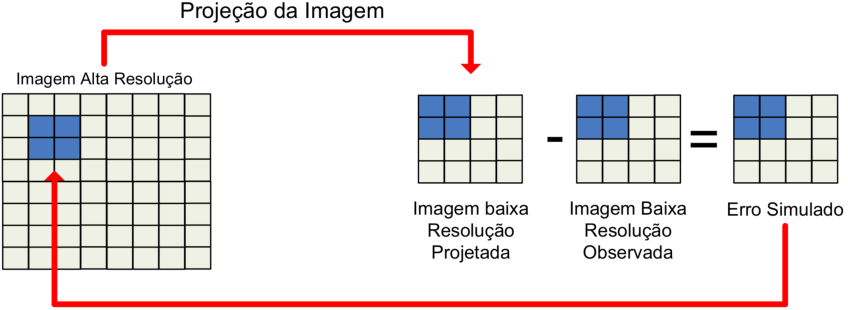
\includegraphics[width=.97\textwidth]{./figures/ibpdiagram.pdf}
	\legend{Fonte: REIS, 2014 \cite{reis2014metodo}}
\end{figure}

O método parte de um modelo de observação como o apresentado na Seção \ref{sec:obsmodel} no qual uma imagem de baixa resolução $\mathbf{y}^{(k)}$ é dada por

\begin{equation}
	\mathbf{y}^{(k)} = \mathbf{W}^{(k)} \mathbf{x}.
\end{equation}

Onde $\mathbf{x}$ é a imagem de alta resolução a ser encontrada e $\mathbf{W}^{(k)}$ é a matriz que aplica as transformações do modelo de observação.

Se for feito um palpite tanto para a matriz de sistema quanto para a imagem a ser estimada, podemos dizer que o erro do palpite é dado por (\ref{eq:ibperror1}).
Feito isso, a melhor estimativa para a imagem de alta resolução $\mathbf{x}$ seria a que minimiza o erro na Equação (\ref{eq:ibperrorsum}).
Essa estimativa é alcaçada através de métodos iterativos como o de mínimos quadrados.

\begin{gather}
	\label{eq:ibperror1} \mathbf{e}^{(k)}_j = \mathbf{y}^{(k)}-\mathbf{W}^{(k)}_j \mathbf{x}_j \\
	\label{eq:ibperrorsum} \epsilon_j = \sqrt{\sum^N_{k=1}{\|\mathbf{y}^{(k)}-\mathbf{W}^{(k)}_j \mathbf{x}_j\|^2_2}}
\end{gather}

O método \emph{Iterative Back Projections} tem a vantagem de ser intuitivo e de fácil compreensão.
No entanto, ele tem problemas por não ter uma solução única, além de não permitir que se use com facilidade o conhecimento a priori acerca da imagem de alta resolução \cite{nasrollahi2014super, park2003super}.
% SUGGESTION: Inserir figura do esquema de IBP.
% SUGGESTION: Inserir equaçõ do algoritmo de IBP.

\subsection{\emph{Projection Onto Convex Sets}}
Este método de Super-resolução apareceu primeiro no trabalho de Stark e Oskoui \cite{stark1989high}.
O método POCS, assim como o IBP, também é um método iterativo, mas que se diferencia por incorporar um conhecimento \emph{a priori} sobre a imagem. Assume-se que esse conhecimento \emph{a priori} é um conjunto convexo fechado, definido como:
\begin{equation}
	S_{\mathbf{x}} = \{ \mathbf{x} : \delta_i < |\mathbf{y}^{(k)}-\mathbf{W}^{(k)}_j \mathbf{x}_j| < \delta_s \}
\end{equation}
onde $\delta_i$ e $\delta_s$ são os limites superiores in inferiores da incerteza do modelo, respectivamente \cite{nasrollahi2014super}.

A solução do problema $\hat{\mathbf{x}}$ está na intersecção dos conjuntos convexos. A busca pela imagem de alta resolução é feita através do método iterativo abaixo\cite{reis2014metodo}.
\begin{equation}
	\hat{\mathbf{x}}^{n+1} = P_m P_{m-1} ... P_1 P_0 \hat{\mathbf{x}}^{n}
\end{equation}
onde $P$ são operadores de projeção para cada conjunto convexo.

Sobre as vantagens e desvantagens do método de \emph{Projection Onto Convex Sets}, Park et. al dizem:

\begin{citacao}
As vantagens do método POCS são sua simplicidade e o uso poderoso modelo de observação de domínio espacial. O método também permite uma inclusão conveniente de informações a priori. Esses métodos têm as desvantagens de não-singularidade da solução, convergência lenta e um alto custo computacional. \cite{park2003super}
\end{citacao}

\subsection{Máxima Verossimilhança}
\label{sec:metodosprob}

Consideremos o modelo de observação em (\ref{eq:degradation}), onde o vetor
$\mathbf{n}$ representa o ruído adicionado às imagens de baixa resolução.
Sabendo que cada elemento $\mathbf{n}_i$ é aleatório seguindo uma distribuição
gaussiana de média 0 e variância $1/\beta$, podemos estabelecer que a função
densidade de probabilidade de $\mathbf{n}$ é representada em (\ref{eq:noisedensity}).

\begin{equation}
	\label{eq:noisedensity}
	p(\mathbf{n}^{(k)}) = \left(\frac{ \beta}{2\pi} \right)^{M/2}
	\exp{\left\{  -  \frac{\beta}{2}\|\mathbf{n}^{(k)}\|^2 \right\}}
\end{equation}

Ainda baseado em (\ref{eq:degradation}), a relação entre uma estimativa da imagem de alta resolução $\mathbf{x}$ e a imagem de baixa resolução observada é:

\begin{equation}
	\mathbf{y}^{(k)} - \mathbf{W}^{(k)} \mathbf{x} =  \mathbf{n}^{(k)} \\
\end{equation}

Então é possível dizer que a probabilidade de $\mathbf{y}^{(k)}$ ocorrer baseado em uma estimativa da imagem de alta resolução $\mathbf{x}$ é dada pela distribuição em (\ref{eq:ykdistr}).

\begin{equation}
	\label{eq:ykdistr}
	p(\mathbf{y}^{(k)} | \mathbf{x}, \mathbf{W}^{(k)}) = \left(\frac{ \beta}{2\pi} \right)^{M/2}
	\exp{\left\{-\frac{\beta}{2}\|\mathbf{y}^{(k)} - \mathbf{W}^{(k)}\mathbf{x} \|^2 \right\}}
\end{equation}

O logaritmo da função de verossimilhança de $\mathbf{y}^{(k)}$ é expresso em

\begin{equation}
	\mathcal{L}\{\mathbf{y}^{(k)}\} = \log \left[ p(\mathbf{y}^{(k)} | \mathbf{x}, \mathbf{W}^{(k)}) \right]
\end{equation}

Aplicando o logaritmo e eliminando todas as variáveis que não dependem de $\mathbf{y}^{(k)}$ temos que:

\begin{equation}
	\mathcal{L}\{\mathbf{y}^{(k)}\} = -\|\mathbf{y}^{(k)} - \mathbf{W}^{(k)}\mathbf{x}\|^2.
\end{equation}

Teoricamente, a melhor estimativa ($\hat{\mathbf{x}}$) da imagem de alta resolução é a
que maximiza a função de verossimilhança acima, como é demonstrado em (\ref{eq:maxlhood}).

\begin{gather}
	\label{eq:maxlhood}
	\hat{\mathbf{x}}_{ML} = \argmax_{\mathbf{x}}
	\left[ - \|\mathbf{y}^{(k)} - \mathbf{W}^{(k)}\mathbf{x}\|^2 
	\right ] \\
	\hat{\mathbf{x}}_{ML} = \argmin_{\mathbf{x}}
	\left[ \|\mathbf{y}^{(k)} - \mathbf{W}^{(k)}\mathbf{x}\|^2 
	\right ] 
\end{gather}


Considerando que o diferencial da função de verossimilhança em relação a $\mathbf{x}$ é dado por:
\begin{equation}
	\frac{\mathrm{d}}{\mathrm{d} \mathbf{x}}
	\mathcal{L}\{\mathbf{y}^{(k)}\} = -2 (\mathbf{y}^{(k)} - \mathbf{W}^{(k)}\mathbf{x}) {\mathbf{W}^{(k)}}^T \\
\end{equation}

Basta igualar a derivada à zero e fazer as devidas manupulações para encontrar o estimador de máxima verossimilhança $\hat{\mathbf{x}}_{ML}$: 

\begin{gather}
	(\mathbf{y}^{(k)} - \mathbf{W}^{(k)}\hat{\mathbf{x}}) {\mathbf{W}^{(k)}}^T = 0 \\
	\hat{\mathbf{x}}_{ML} = (\mathbf{W}^T\mathbf{W})^{-1} \mathbf{W}^T \mathbf{y}^{(k)}
% ISUUE: Corrigir as matrizes W nesta equação.
\end{gather}

O método de máxima verossimilhança é sensível a distúrbios causados por ruídos ou
imprecisões na estimação dos parâmetros de aquisição.
Além disso, se o número de imagens não for suficiente, pode haver mais de uma solução
possível. Esse problema deve ser contornado adicionando conhecimento \emph{a priori} da
imagem.
Esse conhecimento ajuda a restringir o número de respostas possíveis \cite{nasrollahi2014super}.

Uma das formas de adicionar conhecimento \emph{a priori} ao método é transformá-lo em
uma abordagem de máximo \emph{a posteriori}.
O método de Super-resolução Bayesiana estudado neste trabalho é um exemplo de método probabilístico que usa inferência Bayesiana para incorporar conhecimento \emph{a priori} acerca da imagem ao modelo.

\subsection{Máximo a posteriori}
% ISSUE: Redigir sobre o máximo a posteriori.
Esta abordagem aparece em diversos trabalhos, dentre eles \cite{pickup2007bayesian2,pickup2007bayesian} e \cite{tipping2003bayesian}.
Sendo que este último é objeto de estudo nesta monografia.

A abordagem de Máximo a posteriori faz uso do Teorema de Bayes para estimar a imagem
de alta resolução aplicando um 
conhecimento \emph{a priori} junto com a distribuição de probabilidade condicional
das imagens de baixa resolução.

O Teorema de Bayes é um postulado que permite obter uma probabilidade condicional a
partir de outra.
A sua fórmula é uma das ferramentas mais importantes no estudo de probabilidade e
processos aleatórios.
Segundo Therrien e Tummala, “[O Teorema de Bayes] É usado em uma série de problemas que
geralmente ocorrem nas comunicações ou em outras áreas onde decisões ou inferências
devem ser feitas a partir de algum sinal ou dados observados” \cite{therrien2011probability}.

Em uma abordagem de máximo \emph{a posteriori} o conhecimento acerca da imagem de alta resolução $\mathbf{x}$ é incorporado na forma de uma função densidade de probabilidade $p(\mathbf{x})$.
Teoricamente, essa distribuição pode ser de qualquer forma, desde que obedeça os requisitos de uma função de probabilidade.
No entanto, a distribuição Gaussiana é geralmente escolhida por possibilitar manipulações com mais facilidade.


Tendo uma distribuição como a (\ref{eq:ykdistr}) e um conhecimento \emph{a priori} da imagem de alta resolução $p(\mathbf{x})$, é possível usar o Teorema de Bayes para calcular a probabilidade \emph{a posteriori} da imagem de alta resolução \cite{nasrollahi2014super,pickup2007bayesian,pickup2007bayesian2} . Ao que temos:

\begin{equation}
	\label{eq:mapposterior}
	p(\mathbf{x} | \{\mathbf{y}^{(k)}, \mathbf{W}^{(k)}\}) = \frac{p(\{\mathbf{y}^{(k)}\} | \mathbf{x}, \{\mathbf{W}^{(k)}\}) p(\mathbf{x})}
	{p(\{\mathbf{y}^{(k)}, \mathbf{W}^{(k)}\})}
\end{equation}
onde
\begin{equation}
	p(\{\mathbf{y}^{(k)}\} | \mathbf{x}, \{\mathbf{W}^{(k)}\}) = 
	\prod_k p(\mathbf{y}^{(k)} | \mathbf{x}, \mathbf{W}^{(k)})
\end{equation}

A melhor estimativa $\hat{\mathbf{x}}$ da imagem de alta resolução é a que maximiza o numerador em (\ref{eq:mapposterior}).
Aplicamos o logaritmo para simplificar a fórmula, ao que obtemos:

\begin{gather}
	\hat{\mathbf{x}}_{\mathrm{MAP}} = \argmax_{\mathbf{x}} \log \left[ p(\mathbf{x}) \prod_k p(\mathbf{y}^{(k)} | \mathbf{x}, \mathbf{W}^{(k)}) \right] \\
	\hat{\mathbf{x}}_{\mathrm{MAP}} = \argmax_{\mathbf{x}} \left[ \log p(\mathbf{x}) + \sum_k \log p(\mathbf{y}^{(k)} | \mathbf{x}, \mathbf{W}^{(k)}) \right].
\end{gather}
